Het experiment werd uitgevoerd met 17 proefpersonen, 4 vrouwen en 13 mannen.
Leeftijden varieerden van 21 tot 47 jaar oud met een gemiddelde van 30. Slechts
3 personen hadden geen spelervaring. Omdat zowel de groep van vrouwen als de
groep van mensen zonder spelervaring te klein is kunnen deze groepen helaas
niet apart bekeken worden. Maar op het eerste zicht lijkt er geen significant
verschil te zijn in de resultaten van deze groepen.

De geleverde grondplannen uit de vragenlijst kwamen over het algemeen overeen 
met de realiteit, de enige uitzondering hier op was het grondplan van 
proefpersoon 17, zijn kaart was gespiegeld over de as die met de gang mee loopt.

\begin{figure}[h!]
    \centering
    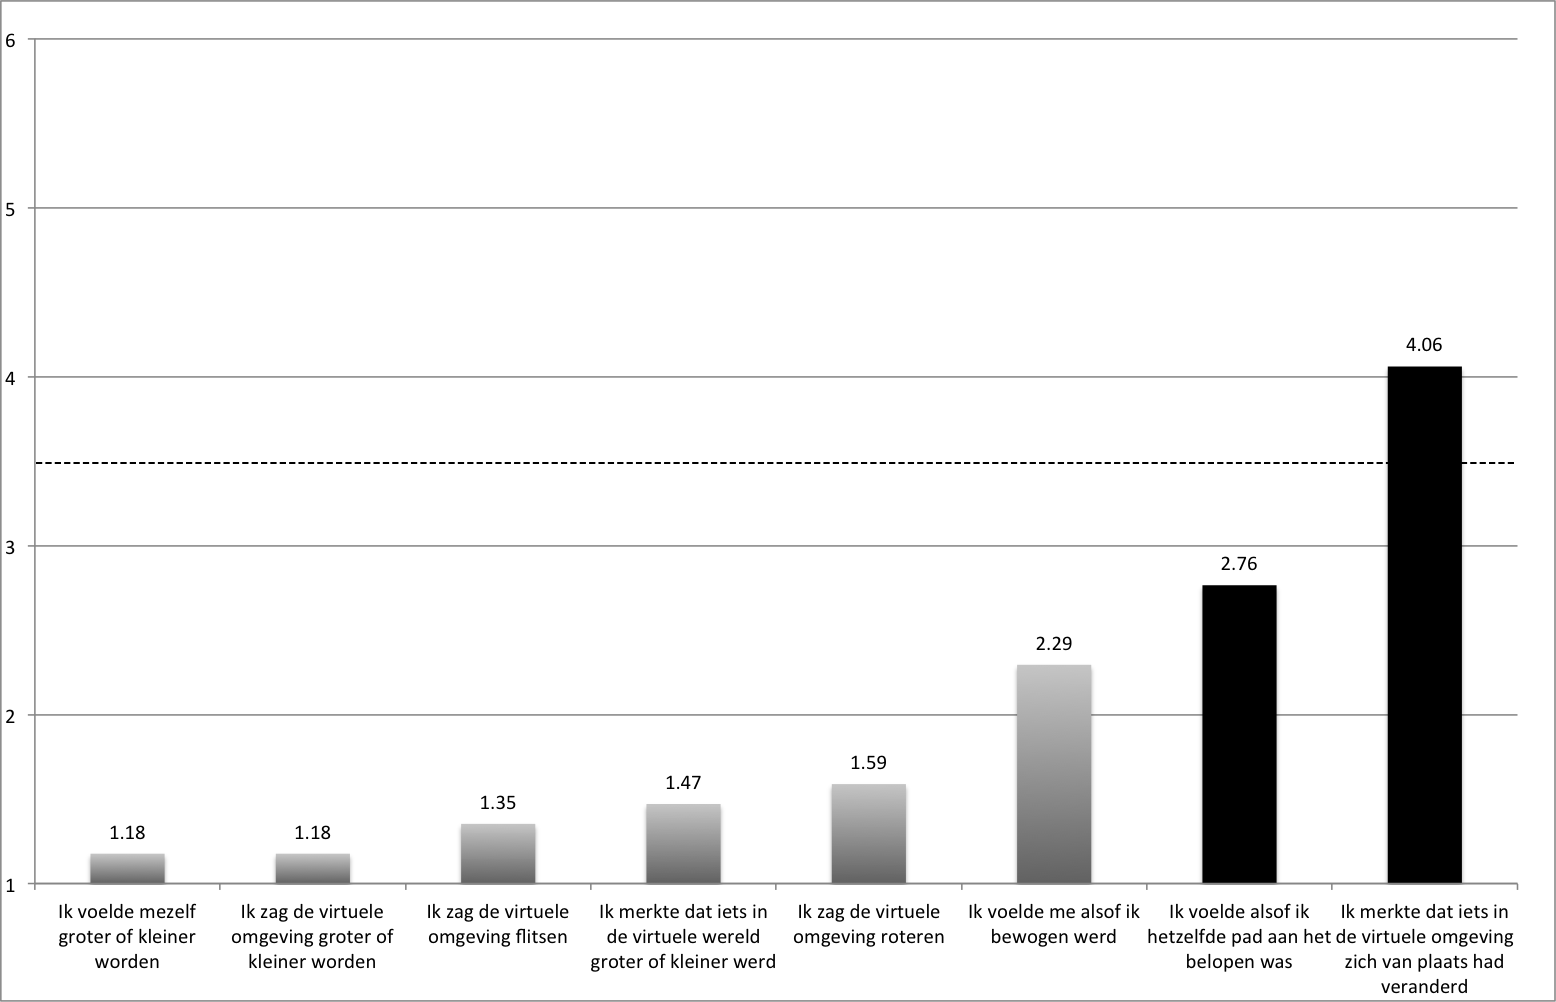
\includegraphics[width=\textwidth]{chart}
    \caption{Grafiek van de gemiddelde scores van de stellingen, de zwarte 
    kolommen zijn de ware stellingen. De stippellijn duidt 3.5 aan, de gemiddelde
    waarde.}
    \label{fig:chart}
\end{figure}

Scores voor de afleidingsstellingen vari\"eren tussen 1.18 en 2.29, de hoge score
van ``Ik voelde me alsof ik bewogen werd'' valt hier op. Vermoedelijk werd die
vraag door sommigen verkeerd ge\"interpreteerd, het zou ook kunnen dat de 110\%
snelheidsschalering werd opgemerkt door de proefpersonen. Zowel ``Ik voelde alsof 
ik hetzelfde pad aan het belopen was'' ($\bar{x}$: 2.76) als ``Ik merkte dat iets 
in de omgeving zich van plaats had veranderd'' ($\bar{x}$: 4.06) behaalden hoge
gemiddelde scores. Dit duidt aan dat de verplaatsing van de deur eerder wel
merkbaar was, maar dat de aard van het pad door de fysieke omgeving niet zeer
merkbaar was. Hoewel de proefpersonen over het algemeen merkten dat er een 
verandering in de scene gebeurd was, kon slechts 47\% van de proefpersoon
vermelden dat het de deur was die bewogen was.


\section{Bespreking feedback}
Een van de vragen op de vragenlijst vroeg of er iets was dat de immersie breekt.
Er werd hier feedback gegeven op diverse problemen:

\begin{itemize}
  \item Fysieke problemen zoals de grootte van de Oculus Rift, het storen van de
        kabels, en rakelings tegen het doek lopen.
  \item Technische problemen zoals het ontbreken van een realistisch input device
        en de resolutie van de Oculus Rift.
\end{itemize}

Deze problemen zouden in de toekomst kunnen opgelost worden door een nieuwere
versie van de Oculus Rift te gebruiken (deze heeft minder kabels en heeft een
hogere resolutie), door de laptop in een rugzak te steken, en door gebruik te 
maken van Wi-Fi voor de netwerkverbinding. In de toekomst zou het ook een goed 
idee zijn om de kamer op andere manier te verduisteren, daar het doek blijkbaar 
stoorde.

Als laatste heb ik ook feedback gekregen dat er kleine haperingen in de tracking
waren, helaas zijn deze kleine haperingen veroorzaakt door een onvoldoende aantal
cameras en kon ik hier niets aan doen. Wegens een kleine hoeveelheid 
netwerklatency zat er ook een beetje vertraging op de reactiesnelheid van het 
systeem. Een van de proefpersonen was ook te groot voor de tracking setup en 
moest een beetje gebukt door de omgeving lopen. Enkele van de proefpersonen die 
de verplaatsing van de deur merkten noteerden dit ook als immersiebrekend, 
vermoedelijk omdat de deur niet meer stond waar ze deze verwachtte.


\section{conclusie}
Het is opvallend dat mijn implementatie vergeleken met eerder onderzoek zoals dat 
van Evan A. Suma \cite{suma11} minder effectief lijkt. Ik kan enkel vermoedens
voorleggen betreffende de oorzaak hiervan. Ik vermoed dat mijn veranderingen te 
extreem zijn vergeleken met het eerder uitgevoerde onderzoek van Evan A. Suma 
\cite{suma11}. In dat onderzoek werd enkel de ori\"entatie van de deur in de hoek 
van de kamer veranderd, terwijl ik deze over de volledig lengte van een muur 
verschuif. Het zou ook kunnen komen door een immersieprobleem zoals de laptop 
die door de uitvoerder van het experiment moet rondgedragen worden of de blinde 
plekken in de tracking area wegens een gebrek aan camera's.

In een verder onderzoek zou getest kunnen worden hoe extreem een verandering in
de scene mag zijn voor deze opvalt. Er zou ook kunnen onderzocht worden wat de
invloed van immersie is op de effectiviteit van change blindness.

Verder zou het mogelijk zijn om change blindness met andere technieken te
combineren zoals rotationele en dynamische translationele vervorming zoals
besproken in de literatuurstudie. Indien alle beschikbare technieken worden 
gecombineerd zou het zelfs mogelijk kunnen zijn een algemeen toepasbare 
redirectietechniek te ontwikkelen die met elke arbitraire virtuele omgeving en 
fysieke ruimte werkt.